\chapter{Modélisation objet}

\secdiagramme{Diagramme de classes de conception}{Conception}{UML 2.5}{Class diagram, Diagram of Implementation Classes}
\label{sec:dcc}
\index{Diagramme de classes}

L'un des diagrammes centraux et le plus utilisé pour la modélisation des systèmes objets est le \gls{diag-cc} (\acrshort{DCC}). Ce diagramme joue le rôle d'une carte du système. On y représente tous les types définis dans le système (\gls{classe}, \gls{interface}, \gls{enumeration}, \gls{structure} ...) ainsi que les composantes de ces types et les relations entre les types. Dans un cycle de conception logicielle, la production du \acrshort{DCC} vient souvent en dernier dans l'étape de la conception tout juste avant de passer à l'implémentation.

Cette section présente la notation \acrshort{UML} pour le \acrshort{DCC} ainsi que des exemples de mise en oeuvre des diagrammes dans le langage de programmation C\#.

\subsection{Définition des types et des méthodes}
\label{ssec:dcc-type-methode}

\index{Diagramme de classes!définition des types}
\index{Diagramme de classes!classes}

La définition d'un type se fait avec une boîte séparée verticalement en trois sections. La section du haut contient la spécification du type ainsi que son nom en caractères gras. Spécialement pour la \gls{classe} il n'y a pas de spécification de type particulière à faire. La section du milieu contient les \glspl{attribut} de la classe et est identifiée par le titre \term{attribut}. La section du bas contient les \glspl{methode} de la classe et est identifiée par le titre \term{operation}.

\begin{figure}[H]
	\caption{Représentation d'une \gls{classe} sur un \acrshort{DCC}}
	\centering
	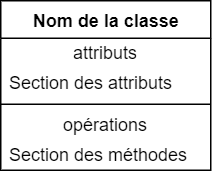
\includegraphics[scale=0.4]{dcc-modele-type.png}
\end{figure}

\index{Diagramme de classes!attribut}
Pour déclarer un \gls{attribut}, il faut indiquer le nom de l'\gls{attribut} suivi du symbole deux-points (:) et du type de la donnée. Les types natifs suivants peuvent être utilisés :

\begin{itemize}
	\item \term{byte} : séquence numérique de bit entre $-2^7$ et $2^7-1$;
	\item \term{char} : représentation d'un caractère sur la table ASCII. Les valeurs permises sont entre $-(2^7)$ et $2^7-1$;
	\item \term{short} : entier court dont la valeur est entre $-2^{15}$ et $2^{15}-1$; 
	\item \term{int} : entier dont la valeur est entre $-2^{31}$ et $2^{31}-1$;
	\item \term{long} : entier long dont la valeur est entre $-2^{63}$ et $2^{63}-1$;
	\item \term{float} : représentation d'un nombre décimal à simple précision (encodé sur 32 bits);
	\item \term{double} : représentation d'un nombre décimal avec une double précision (encodé sur 64 bits);
	\item \term{boolean} : variable booléenne;
	\item \term{string} : chaîne de caractères à longueur variable.
\end{itemize}

En plus des types natifs, il est possible de faire référence à un type complexe (\gls{classe}, \gls{interface}, \gls{enumeration} ...). On inscrit le nom du type auquel l'on fait référence après le symbole du deux-points (:).\\

\index{Diagramme de classes!constantes}
Pour la déclaration d'attributs à valeur constante, on ajoute le symbole d'égalité (=) après le type de l'attribut qui devrait être constant et la valeur de la constante.

Pour déclarer une méthode, il faut simplement indiquer le nom de la méthode suivi de parenthèses qui contiennent les paramètres de la méthode. Les arguments sont notés comme les \glspl{attribut}, c'est-à-dire en indiquant d'abord le nom du paramètre puis le symbole des deux-points ({\NoAutoSpacing  :}) et le type du paramètre. Finalement, il faut inscrire le symbole des deux points ({\NoAutoSpacing  :}) après la parenthèse fermante des paramètres et le type de retour de la méthode.\\


\index{Diagramme de classes!méthode}
\index{Diagramme de classes!constructeur}
Les méthodes qui ne retournent rien doivent avoir le type de retour \term{void}. Les méthodes de type \glspl{constructeur} ont une notation spéciale qui sera vue plus loin. Pour l'instant, comme un \gls{constructeur} ne retourne rien (même pas \term{void}); on omet le deux-points ({\NoAutoSpacing  :}) et le type de retour. 


\begin{figure}[H]
	\caption{Représentation des \glspl{attribut} et des \glspl{methode} sur un \acrshort{DCC}}
	\centering
	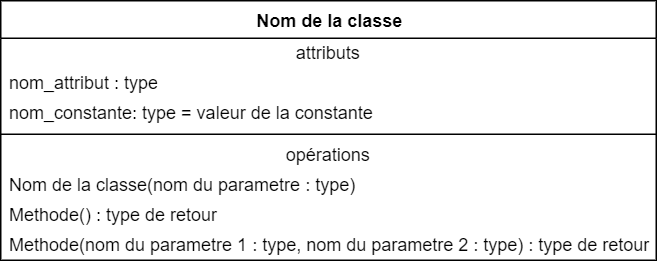
\includegraphics[scale=0.4]{dcc-attributs-methodes.png}
\end{figure}

\begin{exemple}[label = ex:rectangle-1]{La définition classe rectangle}
	
	Dans un système, nous souhaitons développer une classe pour représenter un rectangle. Un rectangle possède une longueur et une hauteur. Il doit définir un constructeur acceptant une longueur et une hauteur, une méthode pour calculer l'aire et une méthode pour vérifier si l'aire du rectangle est plus grande que l'aire d'un autre rectangle. Les valeurs du rectangle seront enregistrées sur le type \term{float}.
	
	\begin{figure}[H]
		\caption{Représentation de la classe Rectangle sur un \acrshort{DCC}}
		\centering
		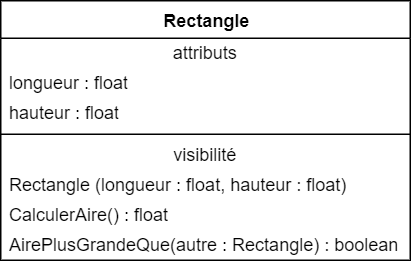
\includegraphics[scale=0.4]{dcc-rect-attributs-methodes.png}
	\end{figure}
	
	\code{Rectangle}{code/rectangle.cs}
	
\end{exemple}

\begin{extra}{Attributs dérivés}
	Un attribut dérivé est un attribut dont la valeur est calculée à partir de la valeur d'autres attributs. Il est possible de noter ces attributs sur le DCC en ajoutant une barre oblique «~/~» devant l'attribut afin de noter le fait qu'il est dérivé à partir d'autres attributs.
\end{extra}

\subsection{Définition de la visibilité}
\index{Diagramme de classes!public}
\index{Diagramme de classes!privé}
\index{Diagramme de classes!protégé}
\index{Diagramme de classes!interne}
\index{Diagramme de classes!visibilité}

Pour chaque membre d'une classe, on peut en préciser la visibilité. Dans le standard UML, il existe quatre types de visibilité. Ces types de visibilité peuvent être partiellement disponibles dans le langage de programmation utilisé (par exemple, le langage C++ définit seulement trois des quatre types de visibilités) ou être interprétés différemment (par exemple, la portée de la visibilité interne en java et en C\# diffère).

Les quatre visibilités disponibles sont :
\begin{itemize}
	\item \term{privé} : le membre est accessible uniquement dans le type où le membre est défini. Les membres privés sont précédés du symbole du trait d'union (-).
	\item \term{protégé} : le membre est accessible uniquement dans les classes \glspl{enfant} du type où le membre est défini. Les membres protégés sont précédés du symbole du dièse (\#).
	\item \term{interne} : le membre est accessible uniquement depuis une portion du système. La portion du système accessible varie selon le langage de programmation. Les membres internes sont précédés du symbole du tilde (\~).
	\item \term{publique} : accessible à tous les autres types du système. Les membres publics sont précédés du symbole plus (+).
\end{itemize}

\begin{figure}[H]
	\caption{Représentation des types de \gls{visibilite} sur un \acrshort{DCC}}
	\centering
	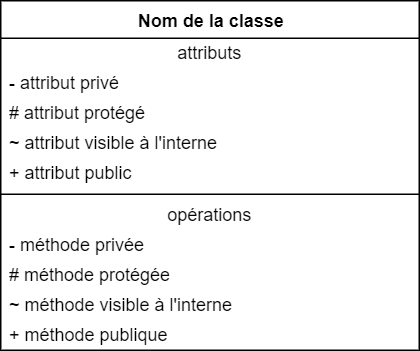
\includegraphics[scale=0.4]{dcc-visibilite.png}
\end{figure}

\begin{exemple}[label = ex:rect-visibilite]{La visibilité des membres de la classe rectangle}
	
	Reprenons la classe rectangle de l'exemple \ref{ex:rectangle-1}. Nous ajoutons l'information sur le diagramme que les attributs de la classe sont \term{privés} et que ses méthodes sont \term{publiques}. À l'exemple \ref{ex:XXX} nous présenterons la visibilité \term{protégée} et son impact.
	
	\begin{figure}[H]
		\caption{Représentation de la classe Rectangle sur un \acrshort{DCC}}
		\centering
		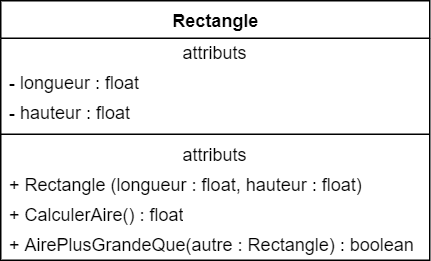
\includegraphics[scale=0.4]{dcc-rect-visibilite.png}
	\end{figure}
	
	\code{Rectangle}{code/rect-visibilite.cs}
	
\end{exemple}


\begin{extra}{Visibilité des types}
	Qu'en est-il de la visibilité des types ? Par exemple on écrit souvent \mintinline{csharp}{public class ...} dans le code. Comment représenter la visibilité des classes sur un diagramme UML ?\\
	
	On utilise d'autres types de diagrammes que le \acrshort{DCC} pour ce type de modélisation, dont le diagramme de \term{packages} ou le diagramme de \term{composites}. Si l'information de la visibilité d'un type doit à tout prix se retrouver sur un \acrshort{DCC}, il est possible d'utiliser les commentaires (voir section \ref{ssec:dcc-commentaires} pour apprendre comment intégrer des commentaires).
\end{extra}

\subsection{Interfaces, énumérations et structures}

\index{Diagramme de classes!interface}
\index{Diagramme de classes!interface|seealso{définition des types}}
\index{Diagramme de classes!énumération}
\index{Diagramme de classes!énumération|seealso{définition des types}}
\index{Diagramme de classes!structure}
\index{Diagramme de classes!dataType}
\index{Diagramme de classes!structure|seealso{définition des types}}

Pour définir des types de données autres que les classes, il faut préciser à l'aide d'un mot-clé au-dessus du nom du type s'il s'agit d'une interface, une énumération ou une structure. Les mot-clés sont présentés entre une paire de chevrons ($<<\ \ >>$).

\begin{itemize}
	\item \term{dataType} : ce type indique une structure (classe dont les données sont passées par valeur et non par référence).
	\item \term{énumération} : ce type définit un ensemble fini de valeurs possibles pour le type. Selon les langages, il peut y être permis d'y définir des méthodes ou non.
	\item \term{interface} : ce type spécifie des opérations qui doivent être définies par les types implémentant l'interface. Selon les langages, il peut y être permis d'y définir des attributs.
\end{itemize}

\begin{figure}[H]
	\caption{Représentation des différents types de données sur un \acrshort{DCC}}
	\centering
	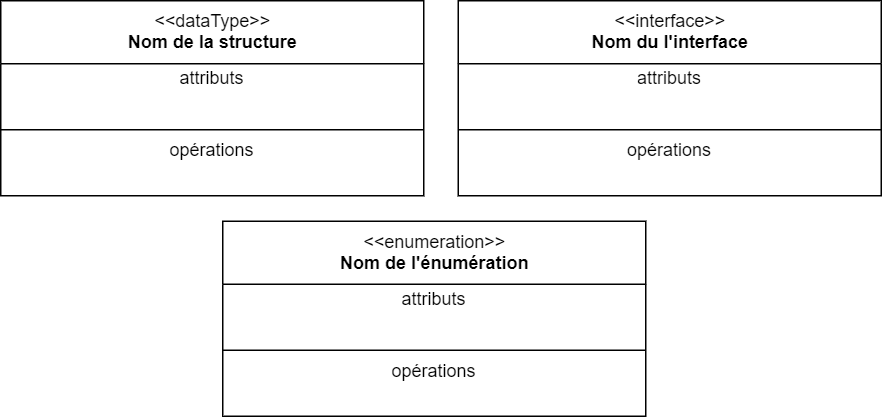
\includegraphics[scale=0.4]{dcc-struct-interface-enum.png}
\end{figure}

\index{Diagramme de classes!stéréotypes}
\begin{distinction}{mot-clés}{stéréotypes}
	Dans la notation UML, deux éléments se note façon semblable : les mots-clés qui indique un type tel \term{interface} ou \term{énumération}, et les stéréotypes de type. Dans plusieurs sources, les termes utilisés en mot-clé sont présentés comme des stéréotypes alors que ce n'est pas le cas.
	
	Les termes identifiant la nature de la structure de données sont des mots définis dans les spécifications de UML, alors que les stéréotypes, de par leur nature présentée à la section \ref{ssec:dcc-stereotype}, peuvent être ajustés selon les besoins.
\end{distinction}


\subsection{Relations entre types}

Au-delà de la structure interne des types, UML permet d'indiquer les relations entre les types. Chaque relation est représentée par un type de flèche différent afin de pouvoir identifier sa nature sur le \acrshort{DCC}. Les sortes de relations couvertes dans le guide sont :

\begin{enumerate}
	\item Agrégation et composition
	\item Héritage
	\item Implémentation (parfois appelé Réalisation)
	\item Dépendance
\end{enumerate}

\subsubsection{Agrégation et composition}
\index{Diagramme de classes!agrégation}
La relation d'agrégation indique qu'un type possède un attribut du type agrégé. C'est une relation appelée «~est partie de ...~». La relation est illustrée par une ligne entre les deux types avec un losange ouvert du côté du type conteneur (qui possède l'attribut). La relation d'agrégation précise aussi une cardinalité indiquant combien d'éléments sont présents de chaque côté de la relation.

\begin{figure}[H]
	\caption{Relation d'agrégation}
	\centering
	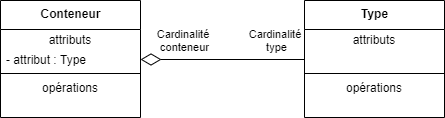
\includegraphics[scale=0.4]{dcc-agregation.png}
\end{figure}

Les cardinalités peuvent être les suivantes :
\index{Diagramme de classes!cardinalités}

\begin{enumerate}
	\item \term{$p$} : indique qu'il y a exactement $n$ éléments d'impliqués (avec $p \geq 1$)
	\item \term{*} : indique qu'il y a 0 ou plusieurs éléments d'impliqués
	\item \term{$p$..$q$} : indique qu'il y a au moins $p$ éléments d'impliqués et au plus $q$ éléments d'impliqués (avec $p \geq 0$ et $q \geq 1$)
	\item si une lettre apparaît dans la cardinalité, alors cela signifie qu'il peut y avoir un nombre quelconque d'éléments impliqués.
\end{enumerate}

\begin{exemple}[label = ex:dcc-cardinalite]{Cardinalité des agrégations}
	
	Voici divers exemples d'agrégations avec la cardinalité utilisée expliquée :
	
	\begin{enumerate}
		\item Une maison possède une adresse. Chaque maison possède une unique adresse donc 1 est indiqué du côté d’adresse, car une seule adresse est impliquée dans la relation. Chaque adresse est unique par maison alors 1 est inscrit du côté de maison, car une seule maison est impliquée dans la relation.
		\begin{figure}[H]
			\caption{Relation d'agrégation entre une maison et son adresse}
			\centering
			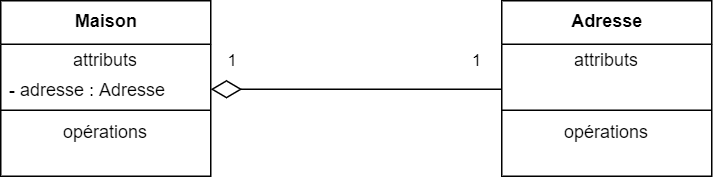
\includegraphics[scale=0.4]{dcc-exemples-agregation-1.png}
		\end{figure}
		
		\item Une automobile comporte entre 0 et 4 roues. Chaque automobile peut avoir entre 0 et 4 roues, donc 0..4 est indiqué du côté de roues. Chaque roue appartient à une seule automobile, alors 1 est indiqué du côté d'automobile.
		
		\begin{figure}[H]
			\caption{Relation d'agrégation entre une automobile et ses roues}
			\centering
			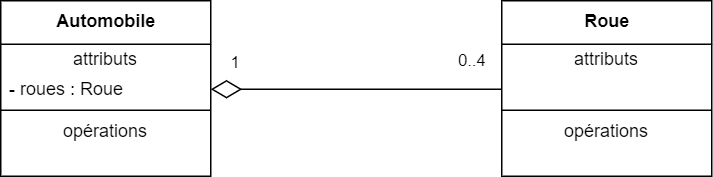
\includegraphics[scale=0.4]{dcc-exemples-agregation-2.png}
		\end{figure}
		
		\item Un panier d'épicerie peut comporter zéro, un ou plusieurs légumes. Comme on peut ne pas mettre de légumes ou en mettre un grand nombre inconnu, * est indiqué du côté de légume. Chaque légume peut être dans un seul panier ou être sur l'étalage (donc dans aucun panier), 0..1 est indiqué à côté de panier d'épicerie.
		
		\begin{figure}[H]
			\caption{Relation d'agrégation entre un panier d'épicerie et les légumes}
			\centering
			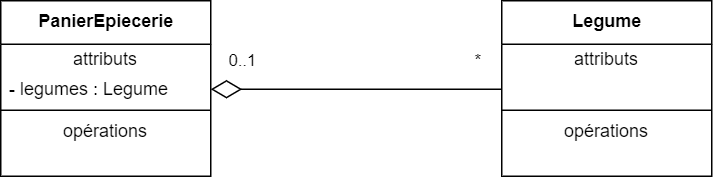
\includegraphics[scale=0.4]{dcc-exemples-agregation-3.png}
		\end{figure}
		
		\item Un groupe doit contenir au moins 6 élèves pour que le cours puisse se donner et ne doit pas en comporter plus de 36. Les valeurs 6..36 est donc indiquée du côté d’élève. Chaque élève doit avoir été inscrit à au moins un groupe (autrement ce n'est pas un élève) et peut être inscrit à un nombre de groupe non limité. La cardinalité 1..n indique que chaque élève se retrouve dans au minimum 1 groupe et peut s'inscrire à plus de groupes.  
		
		\begin{figure}[H]
			\caption{Relation d'agrégation entre un groupe et ses élèves}
			\centering
			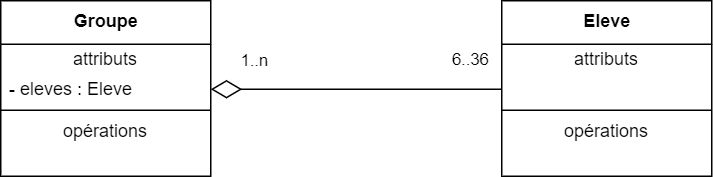
\includegraphics[scale=0.4]{dcc-exemples-agregation-4.png}
		\end{figure} 
		
		\item Chaque entreprise possède au moins un employé et peut en posséder autant qu'elle le souhaite, d'où la notation 1..n utilisée. Une personne employée travaille pour au moins une entreprise (car sinon elle ne serait pas employée) et peut combiner plusieurs emplois en même temps, c'est pouquoi 1..m est indiqué à côté d'entreprise. 
		
		L'utilisation des variables m et n permet de différencier le nombre maximal de personnes employées par entreprise et le nombre maximal d'emplois qu'une personne employée possède.
		
		\begin{figure}[H]
			\caption{Relation d'agrégation entre des entreprises et des personnes employées}
			\centering
			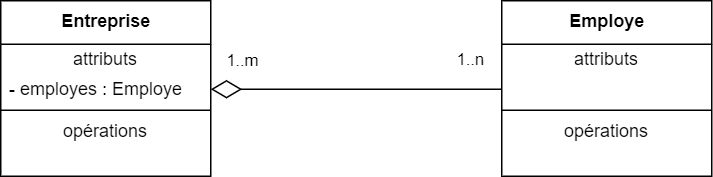
\includegraphics[scale=0.4]{dcc-exemples-agregation-5.png}
		\end{figure} 
		
	\end{enumerate}  
\end{exemple}

\index{Diagramme de classes!composition}
\index{Diagramme de classes!composition|seealso{agrégation}}
La \term{composition} est un type particulier d'agrégation où le conteneur est dépendant de son contenu pour exister. La suppression des éléments contenus entraîne la suppression du conteneur. Dans l'exemple \ref{ex:dcc-cardinalite} la relation illustrée à l'item 4 est une relation de composition. On représente une relation de composition par l'utilisation de la même flèche que pour l'agrégation, mais le losange est plein (au lieu du losange vide).\\

Par exemple, retirer les élèves du groupe entraîne éventuellement la fermeture du groupe. Donc il ne s'agit pas simplement de supprimer un élément contenu pour entraîner la destruction du conteneur, mais bien d'en supprimer toutes les parties. Cette relation contraste avec celle du panier d'épicerie et des légumes (item 2 de l'exemple \ref{ex:dcc-cardinalite}) où même si tous les légumes sont retirés du panier, le panier continue d'exister.

\begin{figure}[H]
	\caption{Relation de composition entre des groupes et des élèves}
	\centering
	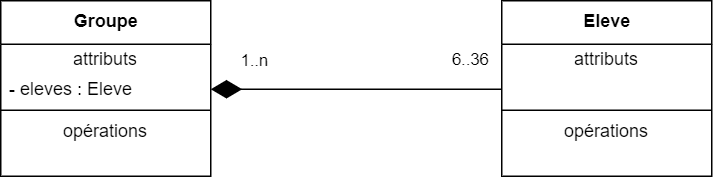
\includegraphics[scale=0.4]{dcc-exemples-composition-1.png}
\end{figure} 

\subsubsection{Héritage}
\label{sssec:heritage}
\index{Diagramme de classes!héritage}

La relation d'héritage permet à un type enfant de reprendre intégralement le contenu d'un autre type appelé parent. On représente la relation d'héritage à l'aide d'une flèche pleine avec une tête triangulaire vide. La tête de la flèche est toujours du côté du type parent (la flèche pointe vers le parent). Lorsqu'un type est hérité par plusieurs autres, il est possible d'utiliser les multi flèches.

On considère que la classe enfant possède tous les attributs et toutes les méthodes de ses parents. Habituellement, ils ne sont pas inscrits de nouveau dans la classe enfant.

\begin{figure}[H]
	\caption{Représentation de la relation d'héritage}
	\centering
	\hfill
	\begin{subfigure}[b]{0.35\textwidth}
		\centering
		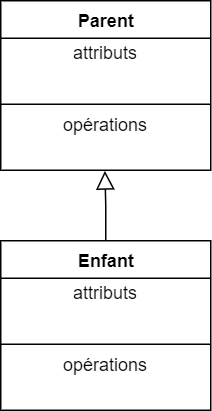
\includegraphics[scale=0.4]{dcc-heritage-simple.png}
		\caption*{Relation d'héritage}
	\end{subfigure}
	\hfill
	\begin{subfigure}[b]{0.5\textwidth}
		\centering
		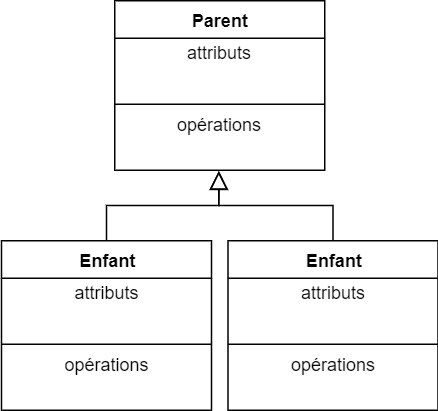
\includegraphics[scale=0.4]{dcc-heritage-multi.png}
		\caption*{Relation d'héritage avec multi flèche}
	\end{subfigure}
	\hfill
\end{figure}

\begin{extra}{Membres hérités}
	Il est possible de noter sur un diagramme les membres héritées d'un parent. Cela peut être utile dans certaines circonstances comme lors d'une redéfinition d'un type générique par exemple (voir section \ref{ssec:generecite}). Lorsqu'on inscrit un membre hérité, on l'écrit dans une couleur gris plus pâle afin de le différencier des membres définis dans la classe enfant.
\end{extra}

\subsubsection{Implémentation}
\index{Diagramme de classes!implémentation}

La relation d'implémentation permet à une classe de réaliser une interface et indique que le type devra implémenter les méthodes spécifiées dans l'interface. La flèche est similaire à celle de l'héritage (voir section \ref{sssec:heritage}), à la différence que le trait est pointillé plutôt que continu. Si plusieurs types implémentent une interface, il est aussi possible d'utiliser une multi flèche.

\begin{figure}[H]
	\caption{Relation d'implémentation entre une interface et un type}
	\centering
	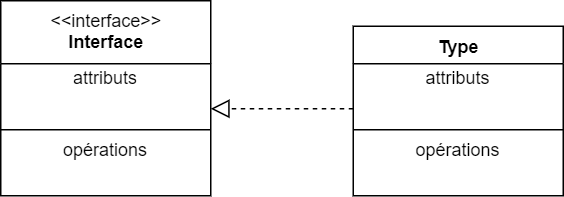
\includegraphics[scale=0.4]{dcc-implementation.png}
\end{figure} 

\subsubsection{Dépendance}
\index{Diagramme de classes!dépendance}
La dépendance entre classes est la relation \acrshort{UML} la moins contraignante. On l'utilise pour indiquer que la modification d'une classe (classe indépendante) peut amener la modification d'une autre classe (classe dépendante). À la différence de la relation d'agrégation, la relation de dépendance ne nécessite pas que la classe dépendante possède un attribut sur l'autre classe. Il faut simplement qu'elle reçoive en paramètre ou qu'elle récupère par un appel de méthode une référence de l'autre classe.

La dépendance dirigée est représentée à l'aide d'une flèche d'un trait plein (certains auteurs présenteront aussi un trait pointillé pour la dépendance). La flèche part du type dépendant vers le type indépendant. Il peut arriver que la dépendance soit bidirectionnelle (donc chacun des types dépend de l'autre), alors une flèche avec deux têtes est utilisée.

\index{Diagramme de classes!agrégation}
Si une relation d'agrégation ou de composition existe déjà entre deux types, la dépendance n'est pas indiquée sur le \acrshort{DCC}, car la relation d'agrégation ou de composition est plus forte que la relation de dépendance.

\begin{bonnepratique}
	\begin{enumerate}
		\item Indiquer toutes les dépendances sur un \acrshort{DCC} crée rapidement une surcharge d'information et un diagramme de type spaghetti. On veut donc se concentrer sur les dépendances les plus importantes afin d'éviter de surcharger le diagramme.
		\item Les dépendances bidirectionnelles sont à éviter autant que possible, car elles ajoutent un grand niveau de complexité dans le développement du système.
	\end{enumerate}
\end{bonnepratique}

\begin{exemple}{Système de génération de formes géométriques}
	Dans le diagramme de classes ci-dessous, on remarque que :
	\begin{enumerate}
		\item Les classes \term{Cercle} et \term{Rectangle} héritent de la classe \term{Forme}.
		\item La classe \term{Forme} implémente l'interface \term{Dessinable}, de sorte qu'elle possède une méthode \term{Dessiner}.
		\item La classe \term{Forme} possède un \term{Système de mesure} pour garder dans quelles unités est définie la forme. Chaque \term{Forme} possède un \term{Système de mesure} et chaque \term{Système de mesure} peut être associé à aucune ou plusieurs \term{Forme}.
		\item L'interface \term{IDessinable} est utilisée par la classe \term{Image}, car \term{Image} définit une méthode dont l'un des paramètres est de type \term{Dessinable}.
		\item La structure \term{Resolution} est utilisée par l'interface \term{IDessinable}. 
		\item La classe \term{Image} agrège des objets de la structure \term{Resolution}. Notons ici que seule l'agrégation est représentée, même si une méthode de la classe \term{Image} possède un paramètre de type \term{Resolution}.
	\end{enumerate}
	
	\begin{figure}[H]
		\caption{\acrshort{DCC} du système de géométrie}  
		\centering
		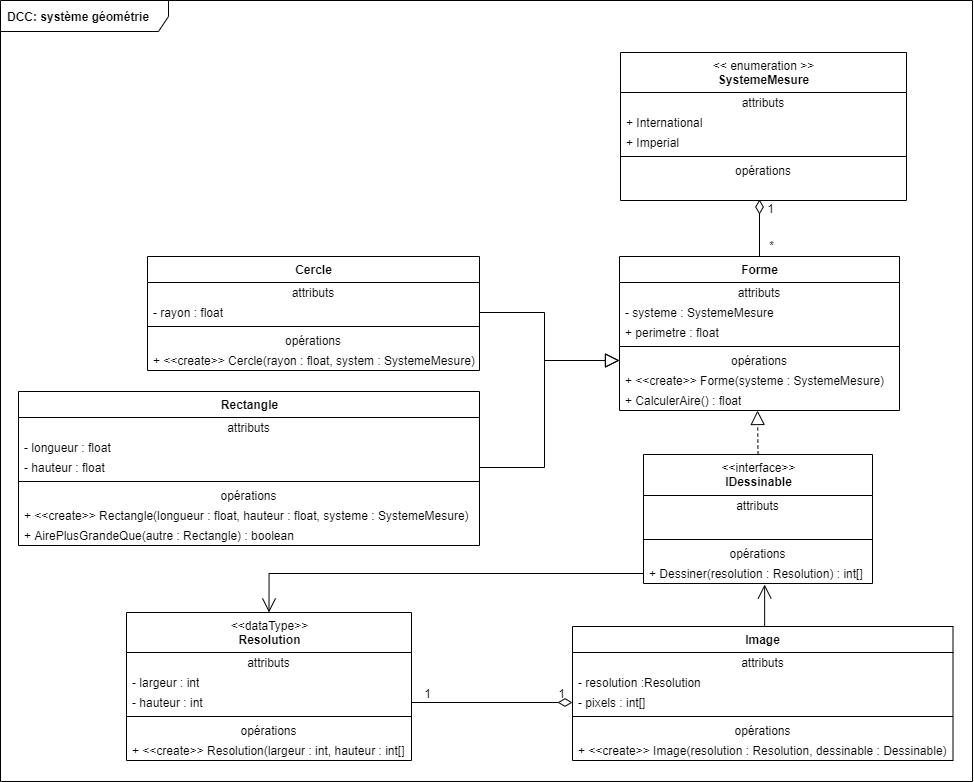
\includegraphics[scale=0.5, angle=90]{dcc-rect-relations.png}
	\end{figure}
\end{exemple}


\subsection{Membres statiques}
\index{Diagramme de classes!statique}
Les membres d'un type peuvent être définis sur le type plutôt que sur ses instances. C'est ce qui est appelé la définition \term{statique} des membres. Dans la notation \acrshort{UML}, les membres statiques sont définis en les soulignant. 

La définition des types statiques est vue à la section \ref{ssec:dcc-stereotype}.

\subsection{Abstraction}
\index{Diagramme de classes!type abstrait}

Les membres abstraits, de même que les types abstraits, sont définis en utilisant {\itshape l'italique} dans leur définition. Les types abstraits définissent uniquement une signature sur le type dans lequel ils sont déclarés et sont implémentés dans l'un des types enfants. Pour un type, être abstrait signifie qu'il ne peut être implémenté.

\begin{exemple}{Membres statiques et abstraction}
	Dans l'exemple ci-dessous, on peut observer les trois particularités suivantes :
	\begin{enumerate}
		\item La constante \term{pi} ($\pi$) est définie dans la classe \term{Cercle}. La constante est définie de façon statique de façon à empêcher sa déclaration pour chaque instance.
		\item L'attribut \term{perimetre} et la méthode \term{CalculerAire} sont définies de façon abstraite dans la classe \term{Forme}. Chaque forme doit donc définir la façon de calculer son périmètre et son aire.
		\item La méthode \term{Dessiner} n'est pas marquée comme abstraite dans l'interface \term{IDessinable}. Comme il s'agit d'une interface, il est attendu que les membres ne définissent pas d'implémentation. Alors ils ne sont pas abstrait strictement parlant et par conséquent ne sont pas marqués en tant que tel.
	\end{enumerate}
	
	\begin{figure}[H]
		\caption{Membres statiques et abstraction dans le système géométrie}
		\centering
		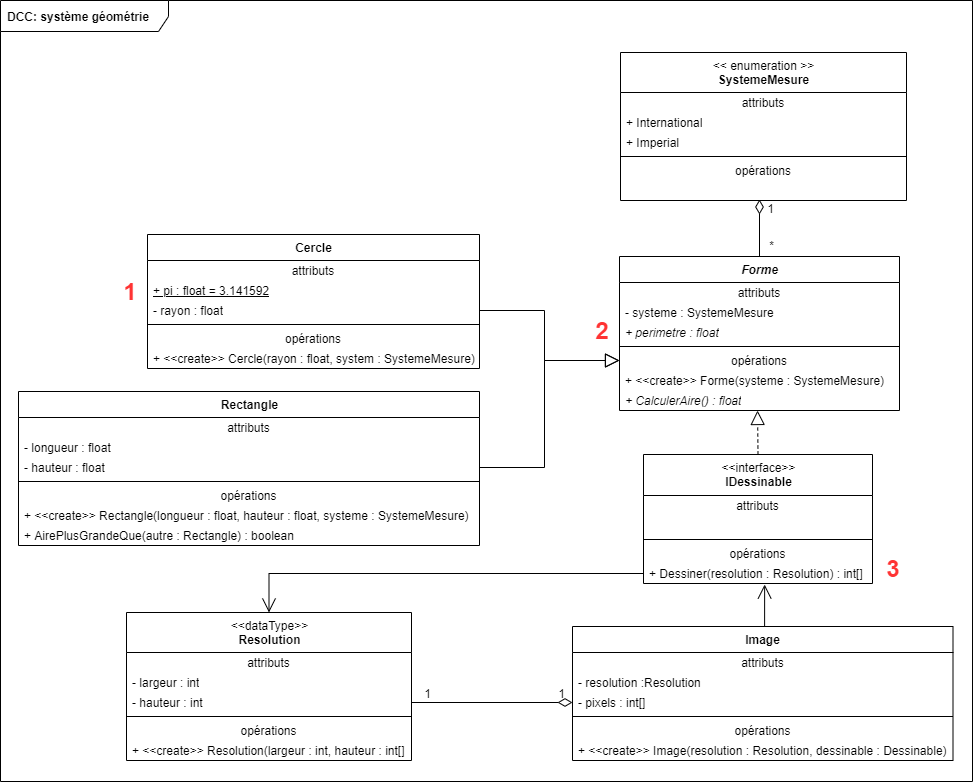
\includegraphics[scale=0.45]{dcc-rect-stat-abs.png}
	\end{figure}
\end{exemple}

\subsection{Stéréotype}
\label{ssec:dcc-stereotype}
\index{Diagramme de classes!stéréotype}

Les stéréotypes servent à indiquer des informations complémentaires sur un type ou un membre. Dans le cadre de ce guide, uniquement les stéréotypes sur les membres seront présentés. Tous les stéréotypes apparaissent entre la visibilité et le nom du membre et ils sont indiqués entre une paire de guillemets français («~»)\footnote{Il est possible d'indiquer une paire de chevrons ($<<\ >>$) si le clavier utilisé ne permet pas d'écrire de guillemets français}. Dans le cadre du guide, deux utilisations des stéréotypes sont présentées la spécification des constructeurs et la spécification de types statiques.

\subsubsection{Constructeurs}
\index{Diagramme de classes!constructeur}
\index{Diagramme de classes!create}

Pour les méthodes, il est aussi possible de renseigner leur utilité à la classe à l'aide d'un stéréotype. Dans le cadre de ce guide, nous identifierons un seul stéréotype : \term{create}.\\

Le stéréotype \term{create} sert à indiquer qu'une méthode crée une nouvelle instance d'un objet. Le stéréotype accompagnera alors tous les constructeurs afin de bien les mettre en évidence. 

\begin{figure}[H]
	\caption{Représentation des stéréotypes sur un \acrshort{DCC}}
	\centering
	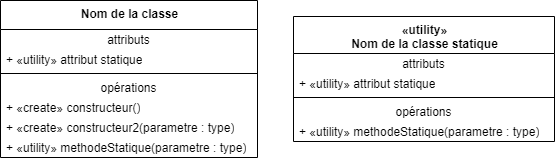
\includegraphics[scale=0.7]{dcc-statique.png}
\end{figure}

\begin{exemple}{Les propriétés de la classe Rectangle}
	En reprenant l'exemple \ref{ex:rect-visibilite}, on transforme les attributs largeur et hauteur en propriétés. On ajoute également deux propriétés. On conserve le système de mesure dans lequel le rectangle est déclaré et on ajoute une propriété appelée Périmètre qui calcule le périmètre du rectangle.
	
	On ajoute aussi le stéréotype \term{create} devant le constructeur afin d'indiquer que cette méthode crée une nouvelle instance du type Rectangle. De cette façon, on sait que l'absence de type de retour (même pas \term{void}) n'est pas une erreur, mais bien le bon comportement.
	
	\begin{figure}[H]
		\caption{Représentation des propriétés de la classe Rectangle}
		\centering
		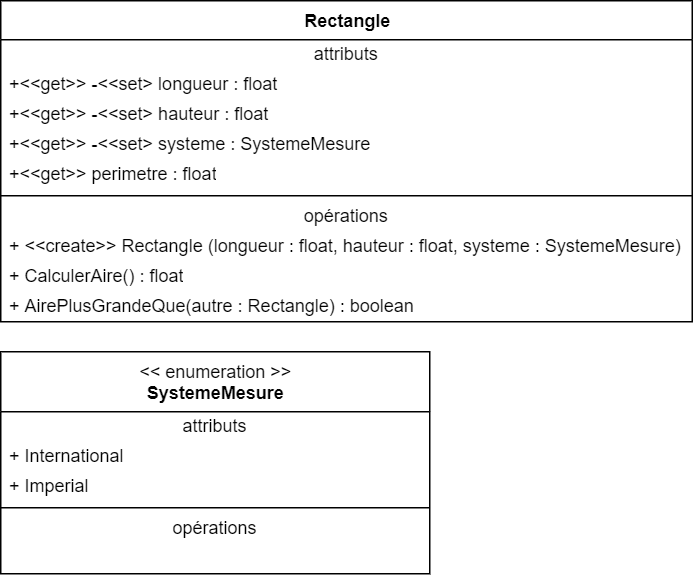
\includegraphics[scale=0.4]{dcc-rect-proprietes.png}
	\end{figure}
	
	\code{Rectangle}{code/rect-proprietes.cs}
\end{exemple}

\subsection{Contraintes}
\label{ssec:dcc-contraintes}
\index{Diagramme de classes!contrainte}

Des contraintes peuvent être appliquées aux membres des classes afin de préciser une particularité ou de préciser une opération interdite. Certaines contraintes utilisent un mot-clé, mais la plupart utilisent la notation de contrainte qui demande d'indiquer entre accolades (\{ \}) le nom de la contrainte utilisée après la signature du type (et la valeur par défaut s'il y a lieu).

\subsubsection{Virtualisation}
\index{Diagramme de classes!virtuel}
\index{Diagramme de classes!virtual}

La contrainte de virtualisation permet d'indiquer qu'un membre (généralement une opération) est virtuel. Un membre virtuel pourra être redéfini, plutôt que masqué, par ses types enfants. Le nom de la contrainte est \term{virtual}.

\subsubsection{Redéfinition}
\index{Diagramme de classes!redéfinition}
\index{Diagramme de classes!redefines}

La contrainte de redéfinition indique qu'un type est redéfini par rapport à son parent. Un membre qui a la même signature que le parent et qui ne possède pas la contrainte de redéfinition est considéré comme masquant son parent. \\

Pour indiquer une redéfinition, on indique la contrainte \term{redefines} suivie du nom du membre du parent qui est redéfini.

\subsubsection{Fermé à la redéfinition}
\index{Diagramme de classes!fermé à la redéfinition}
\index{Diagramme de classes!leaf}

Pour indiquer qu'un membre est fermé à la redéfinition, il faut utiliser la contrainte \term{leaf}.\\

Cette contrainte être utilisé sur un type pour indiquer qu'il n'est pas possible d'en hériter. Dans ce cas, la contrainte est indiquée sous le nom du type.

\subsubsection{Lecture seule}
\index{Diagramme de classes!lecture seule}
\index{Diagramme de classes!readonly}

La contrainte de lecture seule indique que la valeur du membre (généralement un attribut) peut être définie une fois (dans le constructeur pour la plupart des langages) et sera ensuite immuable durant l'exécution. À la différence des constantes, les valeurs en lecture seule ne sont pas assignées à la compilation, mais bien à l'exécution. Le nom de la contrainte de pour la lecture seule est \term{readonly}.

\subsubsection{Autres contraintes}

Les contraintes présentées ici sont quelques-unes des contraintes «~standards~». Bien qu'il n'en existe pas de liste exhaustive, ces contraintes sont suffisamment utilisées, y compris dans la documentation UML, pour les personnes qui utilisent UML comprennent ce à quoi les contraintes font référence.

\subsection{Membres générique}
\label{ssec:genericite}
\index{Diagramme de classes!paramètre générique}

Les paramètres génériques permettent de représenter plusieurs situations directement dans les diagrammes de classe. Les paramètres génériques peuvent être des types, mais peuvent aussi être des valeurs ou des constantes dépendantes de la situation.\\

Pour identifier un paramètre générique sur une classe, on l'indique dans une boîte pointillée située en haut à droite de la classe. Le paramètre générique est identifié d'abord identifié. Ensuite, si l'on souhaite préciser une contrainte sur le type du paramètre générique, on ajoute un deux-points ( : ) puis le type dans lequel le paramètre générique doit être. Finalement, si le paramètre prend une valeur par défaut, on ajoute un symbole d'égalité (=) puis la valeur.

\begin{figure}[H]
	\caption{Représentation de paramètres génériques dans un \acrshort{DCC}}
	\centering
	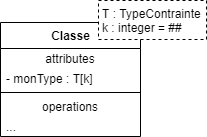
\includegraphics[scale=0.7]{dcc-generique.png}
\end{figure}

\index{Diagramme de classes!type générique}
Lorsqu'un type utilise un type qui définit un paramètre générique (agrégation, implémentation ou héritage), il peut définir une relation de liaison et préciser ou redéfinir la valeur des paramètres génériques. La relation est définie par la mention \term{<<bind>>} suivie du nom du paramètre, d'une flèche ( -> ) et de la nouvelle valeur.

\begin{figure}[H]
	\caption{Représentation de paramètres génériques et de leur spécialisation dans un \acrshort{DCC}}
	\centering
	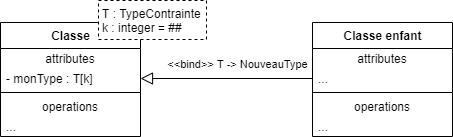
\includegraphics[scale=0.7]{dcc-generique-bind.png}
\end{figure}

\begin{exemple}{Utilisation des génériques}
	On fait la gestion d'un système de file d'attente à la caisse d'une épicerie. On utilise une structure de donnée de type file pour modéliser la situation. En plus des méthodes d'une file standard, on veut pouvoir trouver le client avec le panier le plus plein dans la file afin de possiblement le faire passer à une nouvelle caisse.\\
	
	{\textit Le concept de paramètre générique étant avancé, l'exemple demande des connaissances du cours de} Programmation 3 {\textit pour être compris.}
	
	On remarque sur le diagramme les éléments suivants :
	\begin{enumerate}
		\item Les classes File et Noeud définissent chacune un paramètre générique. Le paramètre générique est de type Objet (donc il doit hériter d’objet). On aurait pu utiliser la même lettre pour désigner le paramètre générique dans les deux classes. Toutefois, dans l'exemple, cela met en évidence que les paramètres génériques sont propres à la visibilité de la classe.
		\item La classe FileClient définit le paramètre générique de T de File comme un client, donc elle utilisera toutes les méthodes de File avec T qui sera toujours un Client.
		\item Le paramètre U de la classe Noeud est toujours défini avec la même valeur que le paramètre T de la classe File lorsque le Noeud est utilisé dans la File. Autrement dit, une File de clients comporte nécessairement des noeuds du type Client. Si la classe Noeud était utilisée dans une autre classe, elle pourrait définir son paramètre U autrement.
	\end{enumerate}
	
	\begin{figure}[H]
		\caption{Système de gestion de file d'attente d'épicerie}
		\centering
		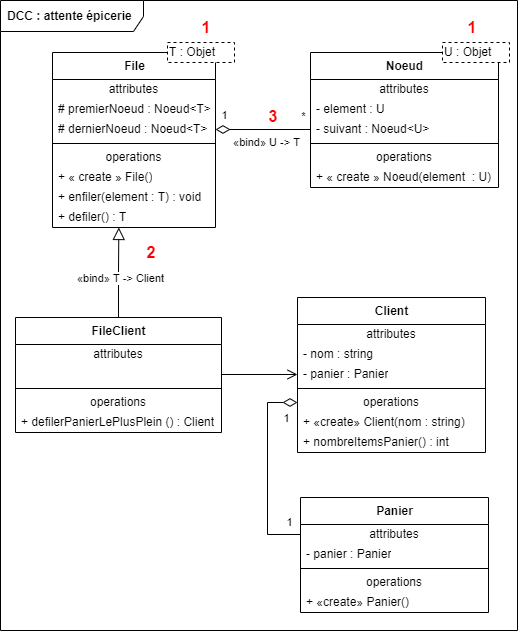
\includegraphics[scale=0.7]{exemple-dcc-file-attente.png}
	\end{figure}
	
\end{exemple}

\subsection{Imbrication}
\index{Diagramme de classes!imbrication}

La relation d'imbrication consiste à définir une classe à l'intérieur d'une autre classe. La classe définie à l'interne peut s'utiliser comme n'importe quelle autre classe du système à partir de la classe dans laquelle elle est définie. Pour le reste du système, la classe interne est vue comme étant dans l'espace de nom de la classe dans laquelle elle est déclarée (comme une variable est dans l'espace de nom de la classe dans laquelle elle est déclarée) avec les limites que cela entraîne.\\

La documentation officielle d'\acrshort{UML} ne précise pas de notation formelle pour la relation d'imbrication de classes. La notation utilisée dans les standards précédents est encore suggérée dans certains contextes. Il s'agit d'une ligne dont la fin est un cercle avec une croix à l'intérieur (appelé ancre). L'ancre est du côté du type englobant.

\begin{figure}[H]
	\caption{Représentation de la relation d'imbrication dans un \acrshort{DCC}}
	\centering
	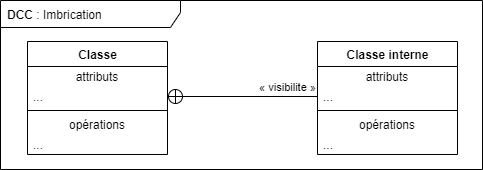
\includegraphics[scale=0.7]{dcc-imbrication.png}
\end{figure}

\subsection{Commentaires}
\label{ssec:dcc-commentaires}
\index{Diagramme de classes!commentaire}

Il est possible de compléter l'information sur un \acrshort{DCC} à l'aide de commentaires. Les commentaires prennent la forme de rectangle avec un coin replié. Un trait pointillé peut indiquer l'élément auquel s'applique le commentaire si le contexte n'énonce pas de façon univoque à quel le commentaire fait référence.


\begin{figure}[H]
	\caption{Commentaire dans \acrshort{DCC}}
	\centering
	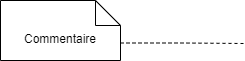
\includegraphics[scale=0.7]{dcc-commentaire.png}
\end{figure}

\secdiagramme{Diagramme d'états-transitions}{Analyse et conception}{UML 2.5}{State diagram}
\label{sec:det}

\hl{Les modèles présentés aux précédentes sections décrivent la structure des classes, mais n'apportent pas de précisions sur les comportements de ces dernières. En UML, il est possible de modéliser les comportements de quatre façons :}

\begin{itemize}
	\item \glspl{diag-etats} d'objets;
	\item diagrammes d'états-transitions de cas d'utilisation;
	\item diagrammes de séquence système;
	\item diagrammes d'activité (diagramme de séquence ou de collaboration).
\end{itemize}

Dans ce guide, seuls les diagrammes d'états-transitions d'objet, qui seront simplement appelés diagramme d'états-transitions (\acrshort{DET}), sont présentés. \index{Diagramme d'états-transitions} Les \glspl{diag-etats} permettent de présenter les différents états dans lesquels un objet peut se retrouver ainsi que les changements qui peuvent être apportés sur cet objet afin qu'il passe d'un état à un autre. 


\subsection{Les états de comportement}

Les états simples sont notés par une boîte arrondie. Le nom de l'état apparaît en {\bfseries gras} dans la boîte. Le nom de l'état est un descriptif (idéalement d'un seul mot) qui indique l'état de l'objet. De règle générale, les états seront nommés selon des adjectifs ou des expressions descriptives tels «~actif~», «~innactif », «~en attente~», «~validé~».

\begin{figure}[H]
	\caption{Représentation d'un état simple dans un \acrshort{DET}}
	\centering
	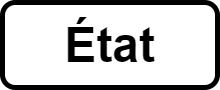
\includegraphics[scale=0.2]{etat1.png}
\end{figure}

On peut aussi ajouter une boîte d'action \index{Diagramme d'états-transitions!action} en dessous du nom de l'état pour indiquer des actions à prendre dans le système lorsque l'objet entre, qu'il demeure ou qu'il sort de l'état. On indique les conditions d'exécution de l'action suivies d'une barre oblique et de la description de l'action. Les trois mots-clés suivants sont employés pour désigner les conditions d'exécution :

\begin{itemize}
	\item \term{entry}\index{Diagramme d'états-transitions!entry} : exécuter lorsque l'objet entre dans l'état;
	\item \term{do}\index{Diagramme d'états-transitions!do} : exécuter tant que l'objet demeure dans l'état;
	\item \term{exit}\index{Diagramme d'états-transitions!exit} : exécuter lorsque l'objet sort de l'état.
\end{itemize}

Si un état n'a pas d'action, alors il s'agit d'un état simple. Il est possible de répéter une condition d'exécution s'il y a plusieurs actions à faire dans une même condition d'exécution (par exemple, s'il y a deux traitements à faire à l'entrée, on indique deux lignes \term{entry}).

\begin{figure}[H]
	\caption{Représentation d'un état avec des actions dans un \acrshort{DET}}
	\centering
	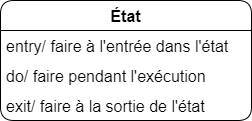
\includegraphics[scale=0.4]{etat2.png}
\end{figure}

\subsubsection{Les superétats}
\index{Diagramme d'états-transitions!Superétat}

Il arrive que certains états puissent partager des caractéristiques ou décomposer un traitement en plusieurs sous-traitements. Prenons l'exemple d'une validation à plusieurs étapes. Il est intéressant alors de regrouper plusieurs états dans un même état appelé \term{superétat}.\\

Un super état est représenté par une boîte semblable à celle d'un état avec des actions, mais contient d'autres états et des transitions au lieu de contenir des actions. Le nom de l'état sera affiché dans une étiquette rectangulaire située en haut à gauche de la boîte. Pour entrer ou sortir d'un super état, il faut utiliser les états spéciaux des superétats présentés à la section \fullref{subsec:etats_speciaux}.

\begin{figure}[H]
	\caption{Représentation d'un superétat dans un \acrshort{DET}}
	\centering
	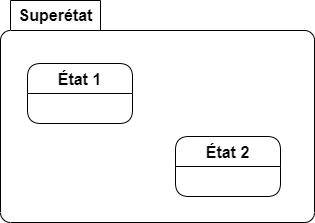
\includegraphics[scale=0.4]{superetat.png}
\end{figure}

\begin{extra}{Notation alternative}
	Il est possible de noter les états  de comportement avec la notation d'une boîte surmontée d'une étiquette (comme pour les superétats). De même, il est possible de noter les superétats avec une simple boîte et un séparateur comme pour les états.
\end{extra}

\subsection{Les transitions}

Les transitions \index{Diagramme d'états-transitions!transition} représentent la possibilité de passer d'un état à un autre. Ils sont représentés par une flèche débutant à un état et se terminant à un autre état. Un texte apparaît toujours sur la flèche indiquant l'élément qui déclenche la transition. 

\begin{figure}[H]
	\caption{Représentation d'une transition dans un \acrshort{DET}}
	\centering
	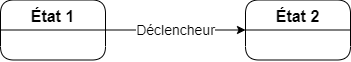
\includegraphics[scale=0.45]{transition-simple.png}
\end{figure}

\subsubsection{Conditions de garde et actions de transition}

Il est aussi possible d'ajouter une condition de garde \index{Diagramme d'états-transitions!condition de garde} pour préciser une condition nécessaire à la réalisation de la transition. Une condition de garde est indiquée entre crochets. Une action peut aussi être effectuée pendant la transition. Si c'est le cas, elle est notée après une barre oblique «~/~». L'ordre d'apparition des thèmes est toujours le suivant :

\begin{center}
	déclencheur [condition de garde]/ action de transition
\end{center}

\begin{figure}[H]
	\caption{Représentation des conditions de garde et des actions de transition dans un \acrshort{DET}}
	\centering
	\hfill
	\begin{subfigure}[b]{0.3\textwidth}
		\centering
		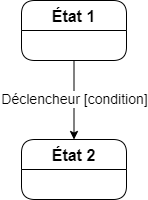
\includegraphics[scale=.45]{transition-condition.png}
		\caption*{Condition de garde}
	\end{subfigure}
	\hfill
	\begin{subfigure}[b]{0.3\textwidth}
		\centering
		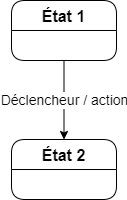
\includegraphics[scale=.45]{transition-action.png}
		\caption*{Action de transition}
	\end{subfigure}
	\hfill
\end{figure}

\begin{important}
	À la sortie d'un état, les conditions doivent être exclusives. C'est-à-dire que pour chaque scénario d'exécution, un seul chemin est disponible. Par exemple les conditions $[x > 10]$ et $[x > 15]$ ne sont pas exclusives, car 20 les satisfait toutes les deux. Par contre, $[10 < x \leq 15]$ et $[x > 15]$ sont des conditions exclusives.\\
	
	Également, {\bfseries il doit toujours y avoir une transition valide pour quitter un état}. Les états spéciaux détruire ou final (voir \ref{subsec:etats_speciaux}) font exceptions à cette règle.
\end{important}

\subsection{Les états spéciaux}
\label{subsec:etats_speciaux}

Les états spéciaux permettent de représenter graphiquement certains états communs à un grand nombre de diagrammes d'états-transitions. Il existe plus d'états spéciaux que présentés ici.

\subsubsection{États dans la vie de l'objet}

Trois états spéciaux servent à décrire la vie d'un objet. 

\begin{itemize}
	\item L'état \term{initial} est le premier état visité dans un \acrshort{DET}. Il indique où commencer à lire le diagramme et représente généralement l'activation ou la création de l'objet. Il est représenté par un cercle vide. \index{Diagramme d'états-transitions!état initial}
	\item L'état \term{détruire} est le dernier état visité dans un \acrshort{DET}. Il indique la destruction de l'objet, et donc, la fin de son comportement. Il est représenté par une croix. \index{Diagramme d'états-transitions!état détruire}
	\item L'état \term{final} est le dernier état visité dans un \acrshort{DET}. Il indique la fin du processus modélisé. À la différence de l'état \term{détruire}, il n'indique pas la destruction de la ressource (ni même sa désactivation), mais simplement la fin du processus. Il est représenté par un cercle plein inscrit dans un plus grand cercle vide. \index{Diagramme d'états-transitions!état final}
\end{itemize}

\begin{figure}[H]
	\caption{Représentation des états spéciaux \term{initial}, \term{détruire} et \term{final} dans un \acrshort{DET}}
	\centering
	\begin{subfigure}[b]{0.3\textwidth}
		\centering
		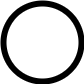
\includegraphics[scale=0.4]{etats-speciaux1.png}
		\caption*{État initial}
	\end{subfigure}
	\hfill
	\begin{subfigure}[b]{0.3\textwidth}
		\centering
		
\includegraphics[scale=0.4]{etats-speciaux2.png}
		\caption*{État détruire}
	\end{subfigure}
	\hfill
	\begin{subfigure}[b]{0.3\textwidth}
		\centering
		
\includegraphics[scale=0.4]{etats-speciaux3.png}
		\caption*{État final}
	\end{subfigure}
\end{figure}

\subsubsection{États de liaisons entre des superétats}
\label{ssubsec:liaisons_superetats}

Sauf exception, il n'existe qu'un point d'entrée dans un superétat. Cela n'exclut pas que plusieurs transitions puissent mener à ce point d'entrée, mais le superétat encapsule ses états internes, donc contrôle le chemin d'accès. Il en va de même pour la sortie du super état. On utilise donc deux états spéciaux pour représenter l'entrée et la sortie d'un superétat.\\

Chacun de ces états est représenté par un symbole placé à la limite du superétat. Une ou plusieurs transitions peuvent provenir ou terminer à ces états spéciaux. Tous les transitions entrantes ou sortantes du super devraient passer par des états spéciaux. Le \term{point d'entrée} \index{Diagramme d'états-transitions!point d'entrée} dans un superétat est représenté par un cercle vide, tandis que le \term{point de sortie} \index{Diagramme d'états-transitions!point de sortie} d'un superétat est représentée par une croix dans un cercle.

\begin{figure}[H]
	\caption{Représentation des états spéciaux \term{point entrée} et \term{point de sortie} dans un superétat de \acrshort{DET}}
	\centering
	~ 
	\hfill
	\begin{subfigure}[b]{0.3\textwidth}
		\centering
		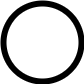
\includegraphics[scale=0.4]{entre-superetat.png}
		\caption*{Point d'entrée}
	\end{subfigure}
	\begin{subfigure}[b]{0.3\textwidth}
		\centering
		
\includegraphics[scale=0.4]{sortie-superetat.png}
		\caption*{Point de sortie}
	\end{subfigure}
	\hfill
	~
	\\
	\begin{subfigure}[b]{\textwidth}
		\centering
		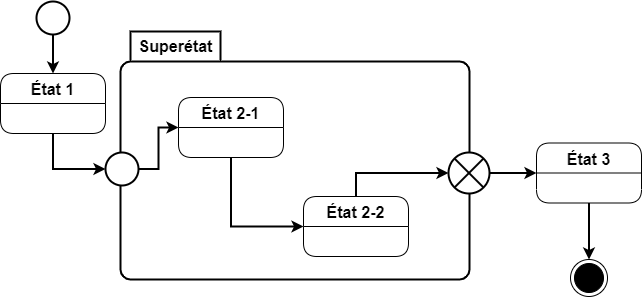
\includegraphics[scale=0.6]{exemple-complet.png}
		\caption*{DET avec un superétat}
	\end{subfigure}
\end{figure}

\subsection{Exemples complets}

\subsubsection{Étude de cas - La machine distributrice}

Une machine distributrice offre différentes boissons aux utilisateurs. Elle doit percevoir le paiement et après remettre la boisson si le montant perçu est le bon. S'il y a trop d'argent inséré, elle doit rendre la monnaie.

\begin{sidewaysfigure}
	\begin{figure}[H]
		\caption{Étude de cas - DET d'une machine distributrice}
		\centering
		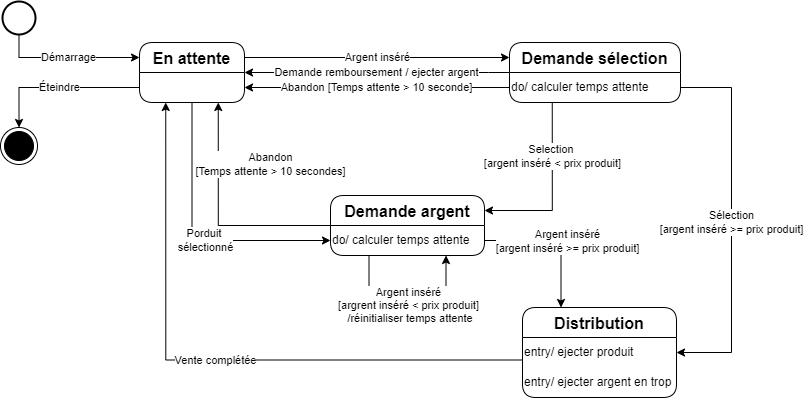
\includegraphics[scale=0.5]{cas-distributrice.png}
	\end{figure}
\end{sidewaysfigure}

\paragraph{À noter sur le diagramme : } 

\begin{enumerate}
	\item Il y a la présence d'un état entrée et d'un état sortie;
	\item Chaque transition est nommée selon l'opération qui lui permet d'être activée;
	\item Chaque état possède une sortie (le système ne peut pas rester pris quelque part);
	\item Chaque chemin est exclusif (on ne pourrait pas se retrouver dans une situation où une action nous amène à choisir entre deux chemin);
	\item Aucun état interne de l'objet n'est indiqué (on ne retient pas le produit sélectionné ou le montant d'argent requis. Ces éléments ne vont pas sur un DET).
\end{enumerate}

\clearpage

\subsubsection{Étude de cas - La remise d'un travail}

Les élèves reçoivent un travail de leur enseignant et doivent complété celui-ci. Une fois remis, l'enseignant corrige et peut demander une révision du français aux élèves si celui-ci est jugé innadéquat. Une fois le travail corrigé il est archivé jusqu'à la fin du délai de révision de note puis détruit.

\begin{sidewaysfigure}
	\caption{Étude de cas - DET d'une remise d'un travail}
	\centering
\end{sidewaysfigure}

\paragraph{À noter sur le diagramme : } 

\subsection{Banque de dépannage}

\question{Mon objet peut être dans deux états en même temps, comment puis-je représenter cette situation ?}

\begin{itemize}
	\item[$\mathbf{\star}$] Tranformer en un superétat l'un des deux états.
	\item Ajouter un nouvel état qui correspond à la situation où l'objet se retrouve dans les états en même temps .
\end{itemize}

%%% www.uml-diagrams.org

